\documentclass[a4paper,11pt]{article}
\usepackage{amsmath,amsfonts,amssymb,amsthm}
\usepackage{graphicx}
\usepackage{fullpage}
\usepackage{caption}
\usepackage{setspace}
\usepackage{hyperref}
\usepackage{enumerate}
\usepackage[all]{xy}
\usepackage[margin=1in]{geometry}
\usepackage{multirow}
\usepackage{bm}
\usepackage[toc,page]{appendix}
\usepackage{geometry}
\usepackage{siunitx}

\usepackage{listings}
\usepackage{color} %red, green, blue, yellow, cyan, magenta, black, white
\definecolor{mygreen}{RGB}{28,172,0} % color values Red, Green, Blue
\definecolor{mylilas}{RGB}{170,55,241}

\geometry{tmargin=0.7in,bmargin=0.7in,lmargin=0.9in,rmargin=0.9in}

\numberwithin{equation}{section}
\newtheorem{thm}{Theorem}[section]
\newtheorem{lem}[thm]{Lemma}
\newtheorem{cor}[thm]{Corollary}
\newtheorem{exa}[thm]{Example}
\newtheorem{prop}[thm]{Proposition}
\newtheorem{defn}[thm]{Definition}
\newtheorem{claim}[thm]{Claim}
\theoremstyle{remark}
\newtheorem*{rem}{Remark}


\newcommand{\Q}{\mathbb Q}
\newcommand{\Z}{\mathbb Z}
\newcommand{\N}{\mathbb N}
\newcommand{\R}{\mathbb R}
\newcommand{\C}{\mathbb C}
\newcommand{\HH}{\mathbb H}
\newcommand{\F}{\mathbb F}


\title{Reinforcement Learning: An Introduction \\ Attempted Solutions \\ Chapter 2}
\author{Scott Brownlie \& Rafael Rui}
\date{}


\begin{document}
%\pagenumbering{gobble}
\maketitle
%\newpage
%\pagenumbering{arabic}

\section{Exercise 2.1}

\textbf{In $\epsilon$-greedy action selection, for the case of two actions and $\epsilon = 0.5$, what is the probability that the greedy action is selected?}
\\ \\
The greedy action is initially selected with probability 0.5, and if not, then one of the two actions is selected randomly (each with probability 0.5). Therefore, the overall probability that the greedy action is selected is
\[
	0.5 + 0.5 \cdot 0.5 = 0.75.
\]


\section{Exercise 2.2: Bandit example}

\textbf{Consider a $k$-armed bandit problem with $k = 4$ actions, denoted 1, 2, 3, and 4. Consider applying to this problem a bandit algorithm using $\epsilon$-greedy action selection, sample-average action-value estimates, and initial estimates of $Q_1(a) = 0$, for all $a$. Suppose the initial sequence of actions and rewards is $A_1 = 1, R_1 = 1, A_2 = 2, R_2 = 1, A_3 = 2, R_3 = 2, A_4 = 2, R_4 = 2, A_5 = 3, R_5 = 0$. On some of these time steps the $\epsilon$ case may have occurred, causing an action to be selected at random. On which time steps did this definitely occur? On which time steps could this possibly have occurred?}
\\ \\
The action value estimates on each time step are as follows:
\begin{enumerate}
	\item $Q_1(1) = 0, Q_1(2) = 0, Q_1(3) = 0, Q_1(4) = 0$
	\item $Q_1(1) = 1, Q_1(2) = 0, Q_1(3) = 0, Q_1(4) = 0$
	\item $Q_1(1) = 1, Q_1(2) = 1, Q_1(3) = 0, Q_1(4) = 0$
	\item $Q_1(1) = 1, Q_1(2) = 3/2, Q_1(3) = 0, Q_1(4) = 0$
	\item $Q_1(1) = 1, Q_1(2) = 5/3, Q_1(3) = 0, Q_1(4) = 0$
	\item $Q_1(1) = 1, Q_1(2) = 5/3, Q_1(3) = 0, Q_1(4) = 0$
\end{enumerate}
The highest actions values on each time step were $\{1,2,3,4\}, \{1\}, \{1, 2\}, \{2\}, \{2\}$ and the chosen actions were $1,2,2,2,3$ respectively.
Therefore, the $\epsilon$ case definitely occurred on time steps 2 and 5. As it is possible that the greedy action is chosen randomly when the $\epsilon$ case occurs, the $\epsilon$ case could possibly have occurred on any of the remaining time steps.


\section{Exercise 2.3}

\textbf{In the comparison shown in Figure 2.2, which method will perform best in the long run in terms of cumulative reward and probability of selecting the best action? How much better will it be? Express your answer quantitatively.}
\\ \\ 
On each time step the probability of selecting the best action is $1-\epsilon$ times the probability that the greedy action is the best action, plus $\epsilon$ times the probability that the best action is chosen randomly. Clearly the probability that the best action is chosen randomly is $1/k$, thus we just need to work out the probability that the greedy action is the best action. 
\\ \\ 
On the first time step all actions have value 0 and we select an action $A_1$ at random and receive a reward $R_1$. Suppose that $R_1 < 0$. What is the probability that $A_1$ is the best action? 


\section{Exercise 2.4}

\textbf{If the step-size parameters, $\alpha_n$, are not constant, then the estimate $Q_n$ is a weighted average of previously received rewards with weighting different from that given by (2.6). What is the weighting on each prior reward for the general case, analogous to (2.6), in terms of the sequence of step-size parameters?}
\\ \\ 
We have
\begin{align*}
	Q_{n+1} & = Q_n + \alpha_n[R_n - Q_n] \\
			& = \alpha_n R_n + (1-\alpha_n) Q_n \\
			& = \alpha_n R_n + (1-\alpha_n)[\alpha_{n-1} R_{n-1} + (1-\alpha_{n-1}) Q_{n-1}] \\
			& = \alpha_n R_n + (1-\alpha_n)\alpha_{n-1}R_{n-1} + (1-\alpha_n)(1-\alpha_{n-1})Q_{n-1} \\
			& = \alpha_n R_n + (1-\alpha_n)\alpha_{n-1}R_{n-1} + \quad \dots + (1-\alpha_n)(1-\alpha_{n-1})\dots (1-\alpha_2)\alpha_1 R_1 + \\
			& \quad \quad (1-\alpha_n)(1-\alpha_{n-1})\dots (1-\alpha_2)(1-\alpha_1) Q_1 \\
			& = Q_1\prod_{j=1}^{n}(1-\alpha_j) + \alpha_n R_n + \sum_{i=1}^{n-1}\alpha_i R_i \prod_{j=i+1}^{n}(1-\alpha_j).
\end{align*}
Therefore, the weighting on $R_n$ is $\alpha_n$ and the weighting on $R_i$ for $i=1,\dots,n-1$ is $\alpha_i \prod_{j=i+1}^{n}(1-\alpha_j)$. Note that when $\alpha_i = \alpha$ for all $i$ the expression above reduces to
\[
	(1-\alpha)^n Q_1 + \alpha R_n + \sum_{i=1}^{n-1}\alpha(1-\alpha)^{n-i}R_i = (1-\alpha)^n Q_1 + \sum_{i=1}^{n}\alpha(1-\alpha)^{n-i}R_i,
\]
which is exactly (2.6).


\section{Exercise 2.5}

\textbf{Design and conduct an experiment to demonstrate the difficulties that sample-average methods have for nonstationary problems. Use a modified version of the 10-armed testbed in which all the $q_*(a)$ start out equal and then take independent random walks (say by adding a normally distributed increment with mean zero and standard deviation 0.01 to all the $q_*(a)$ on each step). Prepare plots like Figure 2.2 for an action-value method using sample averages, incrementally computed, and another action-value method using a constant step-size parameter, $\alpha = 0.1$. Use $\epsilon = 0.1$ and longer runs, say of 10,000 steps.}
\\ \\ 
As we can see from Figure \ref{fig:KArmedBanditNonStationarySampleAveraging}, the sample averaging method chooses the optimal action less than 50\% of the time, even after 10,000 time steps. Using a constant step-size of 0.1 works better, as shown in Figure \ref{fig:KArmedBanditNonStationaryConstantStep} where the optimal action is chosen around 75\% of the time after 10,000 time steps.  The sample averaging method does not work as well because after a significant number of time steps the step-size of $1/n$ becomes very small and the action-value estimates cannot adapt to the non-stationary environment.


\begin{figure}
	\centering
	\caption{Average performance of non-stationary $K$-armed bandit with sample averaging.}
	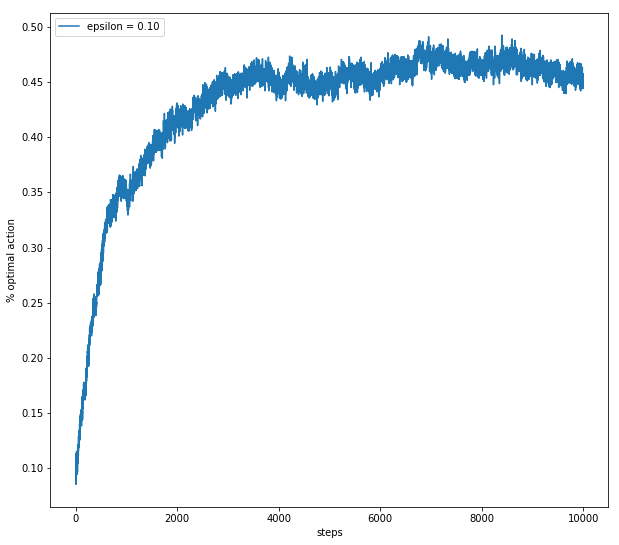
\includegraphics[scale=0.5]{ex2_5_1}
	\label{fig:KArmedBanditNonStationarySampleAveraging}
\end{figure}

\begin{figure}
	\centering
	\caption{Average performance of non-stationary $K$-armed bandit with constant step-size $\alpha=0.1$.}
	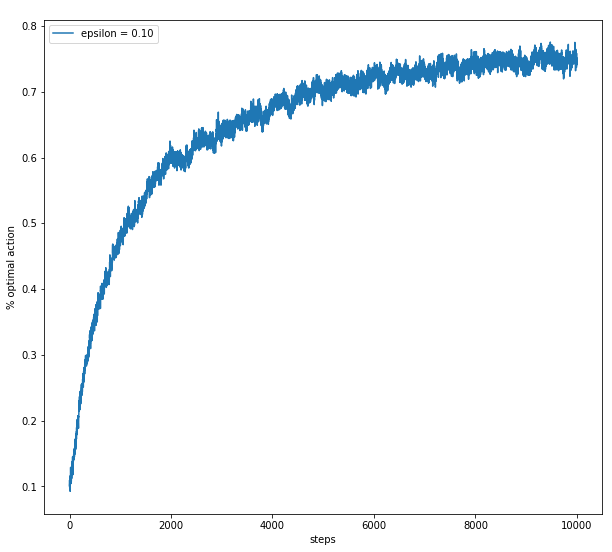
\includegraphics[scale=0.5]{ex2_5_2}
	\label{fig:KArmedBanditNonStationaryConstantStep}
\end{figure}

\end{document}